% !TeX program = pdflatex
\documentclass[border=6pt]{standalone}
\usepackage{amssymb}
\usepackage{tikz}
\usetikzlibrary{arrows.meta, positioning, calc}

\definecolor{MediumRed}{rgb}{0.925, 0.345, 0.345}
\definecolor{MediumGreen}{rgb}{0.37, 0.7, 0.66}
\definecolor{MediumBlue}{rgb}{0.015, 0.315, 0.45}
\definecolor{DarkBlue}{rgb}{0.05, 0.15, 0.35}

\begin{document}
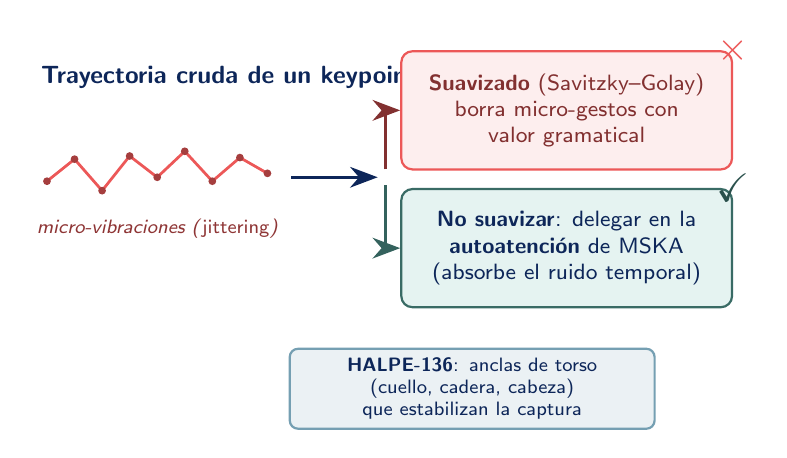
\begin{tikzpicture}[
    font=\sffamily,
    flow/.style={-{Stealth[length=3.5mm]}, line width=1.2pt, DarkBlue},
    opt/.style={draw, thick, rounded corners=4pt, align=center, minimum width=4.2cm,
        minimum height=1.5cm, font=\sffamily\footnotesize},
]

% --- trayectoria cruda con jitter ---
\node[font=\sffamily\small\bfseries, text=DarkBlue, anchor=south west] at (-0.2,1.05)
    {Trayectoria cruda de un \textit{keypoint}};
\draw[MediumRed, line width=1pt]
    (0,0)--(0.35,0.28)--(0.7,-0.12)--(1.05,0.32)--(1.4,0.05)--(1.75,0.38)--(2.1,0.0)--(2.45,0.3)--(2.8,0.1);
\foreach \x/\y in {0/0,0.35/0.28,0.7/-0.12,1.05/0.32,1.4/0.05,1.75/0.38,2.1/0.0,2.45/0.3,2.8/0.1}
    \fill[MediumRed!70!black] (\x,\y) circle (1.4pt);
\node[font=\sffamily\scriptsize\itshape, text=MediumRed!60!black, anchor=north] at (1.4,-0.35)
    {micro-vibraciones (\emph{jittering})};

% flecha de decision
\draw[flow] (3.1,0.05) -- (4.2,0.05);

% --- opcion descartada ---
\node[opt, draw=MediumRed, fill=MediumRed!10, text=MediumRed!55!black] (bad) at (6.6,0.9)
    {\textbf{Suavizado} (Savitzky--Golay)\\ borra micro-gestos con\\ valor gramatical};
% cruz manual (sin dingbats)
\node[text=MediumRed, font=\sffamily\Large\bfseries] at (bad.north east) {$\times$};

% --- opcion elegida ---
\node[opt, draw=MediumGreen!60!black, fill=MediumGreen!16, text=DarkBlue] (good) at (6.6,-0.85)
    {\textbf{No suavizar}: delegar en la\\ \textbf{autoatención} de MSKA\\ (absorbe el ruido temporal)};
\node[text=MediumGreen!45!black, font=\sffamily\Large\bfseries] at (good.north east) {\checkmark};

\draw[flow, MediumRed!55!black] (4.3,0.15) |- (bad.west);
\draw[flow, MediumGreen!55!black] (4.3,-0.05) |- (good.west);

% nota HALPE
\node[draw=MediumBlue!55, thick, rounded corners=3pt, fill=MediumBlue!8, text=DarkBlue,
      font=\sffamily\scriptsize, align=center, text width=4.4cm, below=0.5cm of good, xshift=-1.2cm]
    {\textbf{HALPE-136}: anclas de torso (cuello, cadera, cabeza) que estabilizan la captura};

\end{tikzpicture}
\end{document}
